\section{Conventions de code}
	Par soucis de réutilisabilité et de partage de notre projet, nous avons choisi d'utiliser l'anglais pour la documentation du code mais aussi pour le code en lui-même (nom de fonction, nom de variable, etc).


\section{Répartition du travail}
	La répartition du travail nous a été indirectement imposée par la structure du projet. 
	
	Tout d'abord la partie analyse du projet c'est fait par le groupe entier car
	l'analyse c'est la base d'un projet, donc nous avons choisi de la faire tous ensemble pour essayer d'avoir une analyse représentative du groupe et plus poussée. Comme le projet est divisé en deux parties, la partie développement \gls{android} et la partie \gls{ios}, de ce fait comme seulement Kilian Cousein et Benjamin Tardieu posséder un Macintosh, ces derniers ont développés la partie iOS et l'autre partie à été développée part Olivier Bonvila et Ludovic Pitiot. Enfin en ce qui concerne la partie serveur, c'est Ludovic Pitiot qui l'a implémenté.
	
	
\section{Gestion du projet}
	Pour gérer le projet, nous avons mis en place un serveur \gls{svn} hébergé par GoogleCode (\url{http://code.google.com/p/bomberman-android-ios/}). Nous avons aussi utilisé le wiki et le gestionnaire de problème fourni par GoogleCode.
	
	Ensuite, nous avons fait des réunions pour contrôler l'avancement du projet, environ deux fois par semain. Mais lorsque nous ne pouvions pas ou lorsque que nous avions des problèmes, nous avons utilisé Gmail et son chat.
	

\section{Gestion du temps}
	La réalisation de notre projet se divise en trois axes. Voilà les différents diagrammes de Gantt de ces derniers.
	
	\subsection*{Organisation}
		\begin{center}
			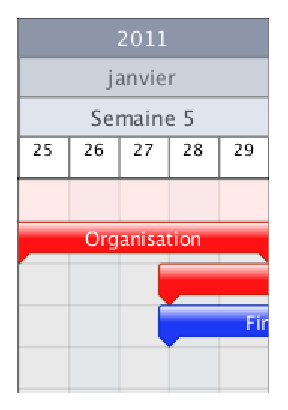
\includegraphics{./Organisation/Img/BomberBlok-Organisation.eps}
		\end{center}
	
	\subsection*{Conception}
		\begin{center}
			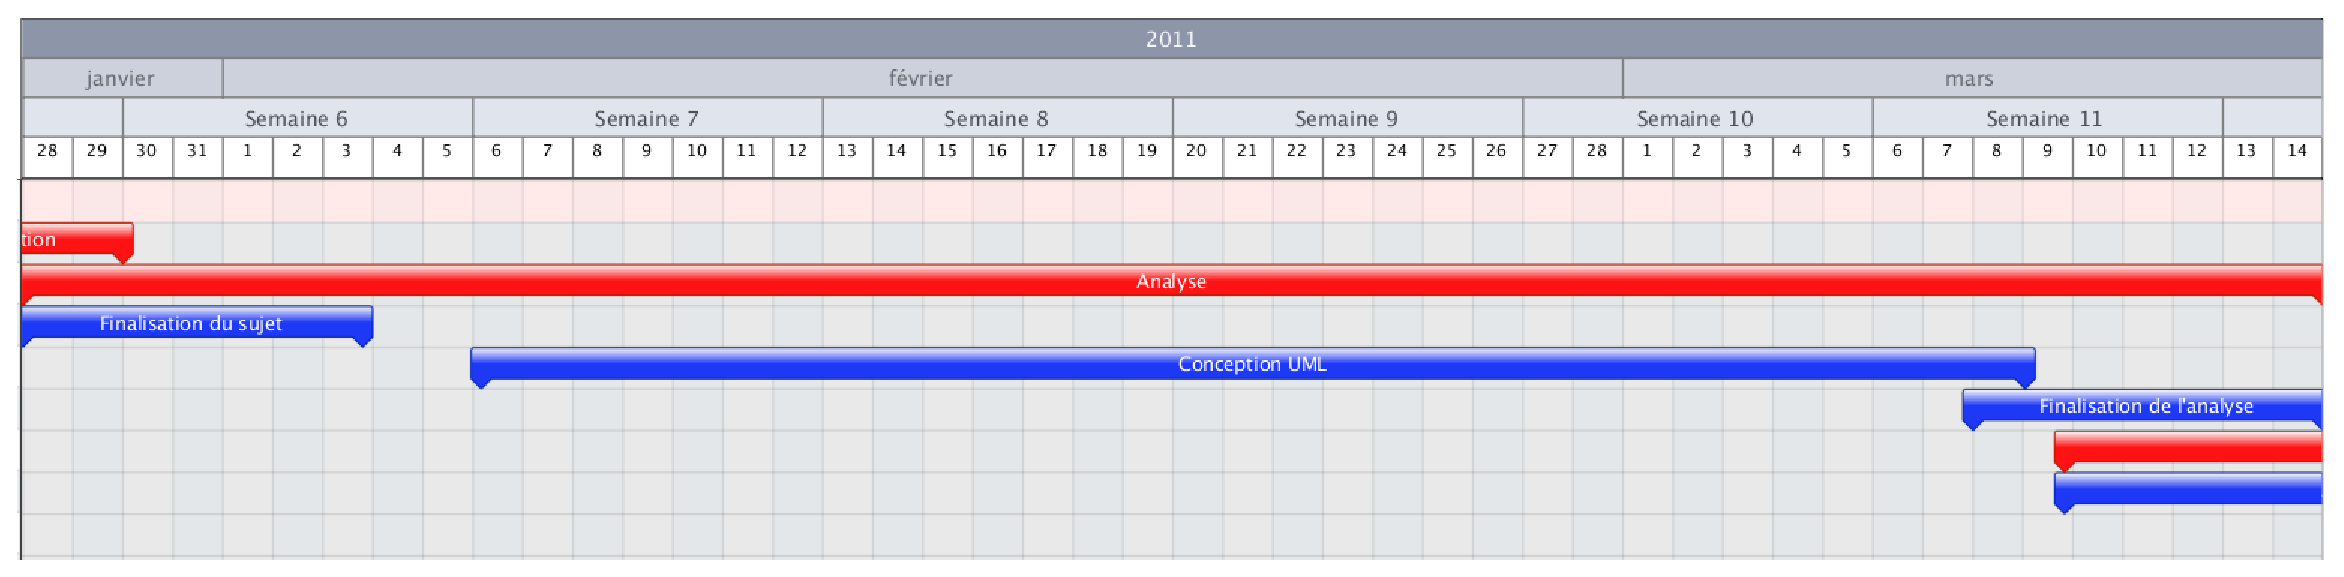
\includegraphics[width=20cm, angle=90]{./Organisation/Img/BomberBlok-Conception.eps}
		\end{center}
	
	\subsection*{Développement}
		\begin{center}
			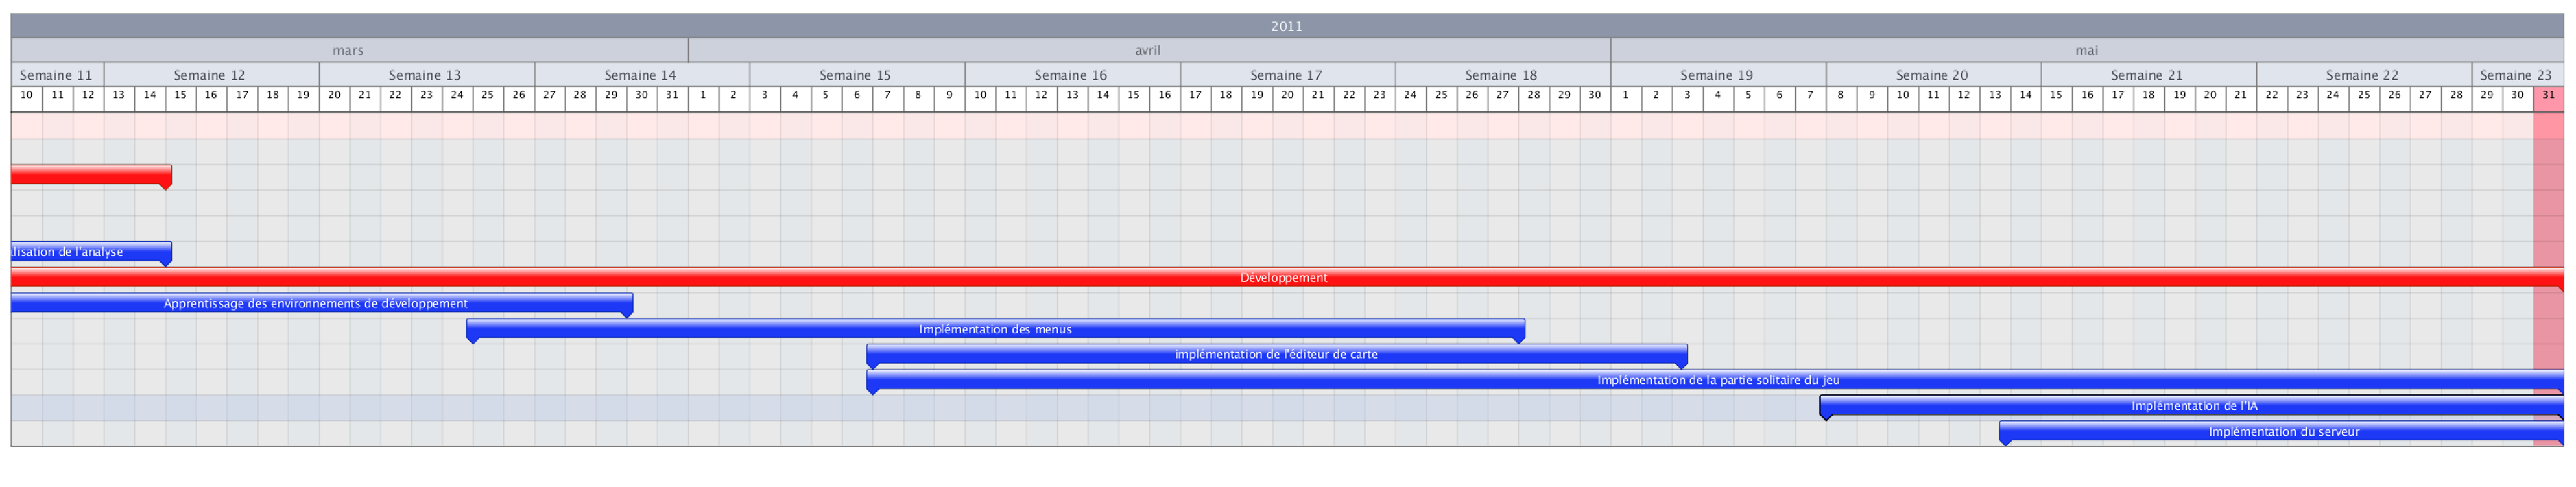
\includegraphics[width=20cm, angle=90]{./Organisation/Img/BomberBlok-Developpement.eps}
		\end{center}